\clearpage
\begin{flushright}
	\textit{Лекция №2}
	\textit{2016.02.15}
\end{flushright}

\begin{figure}[H]
  \centering
  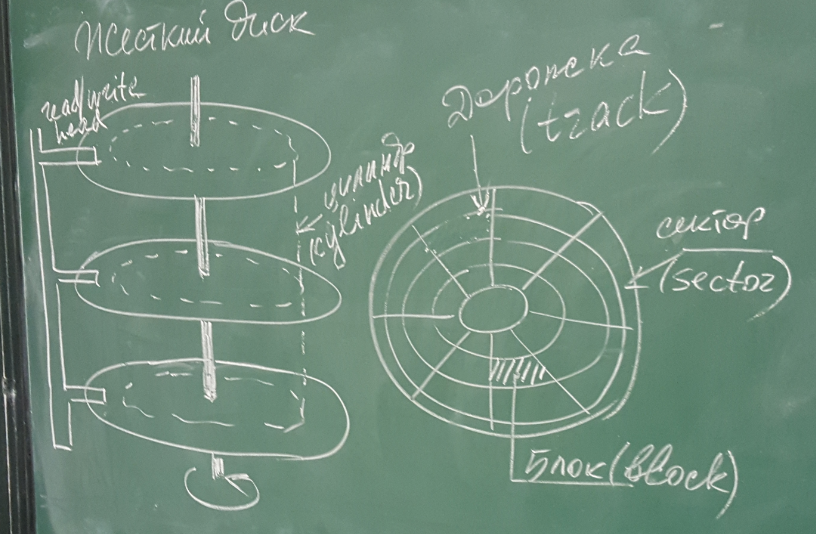
\includegraphics[width=\textwidth]{pic/1.png}
  \caption{Устройство жесткого диска}
\end{figure}

Когда процесс открывает файл, используя $fopen()$, то нужно указать для чего открываем файл. Если для записи, то это широкие права, значит, можем и читать.  С точки зрения системы в программе должен быть создан файловый дескриптор, а система должна позволить нам обрисовать информацию в файле. Файл находится на физическом носителе. Чтобы реализовать действие по доступу процесса к файлу, в системе создается несколько таблиц. Главная таблица – это таблица открытых файлов, в которой хранится информация обо всех файлах, открытых всеми процессами. Таблица – это массив/связный список структур.

\begin{figure}[H]
  \centering
  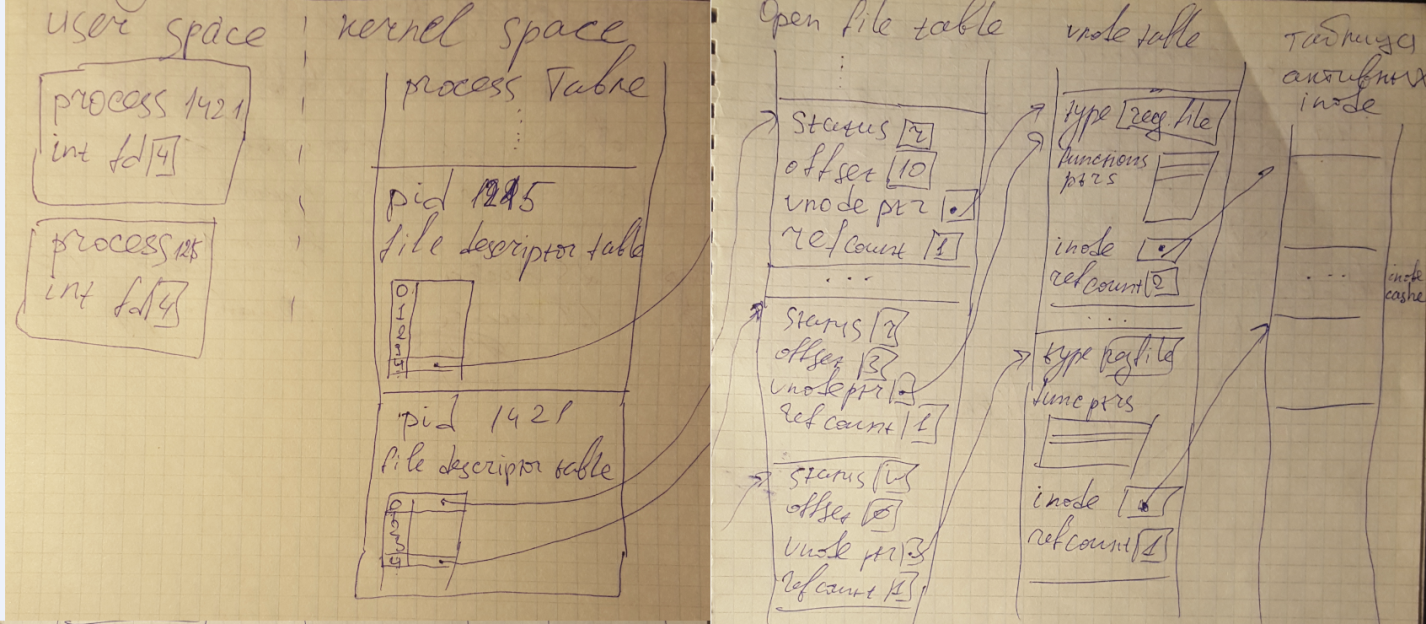
\includegraphics[width=\textwidth]{pic/2.png}
  \caption{Таблицы открытых файлов процессов}
\end{figure}

\begin{figure}[H]
  \centering
  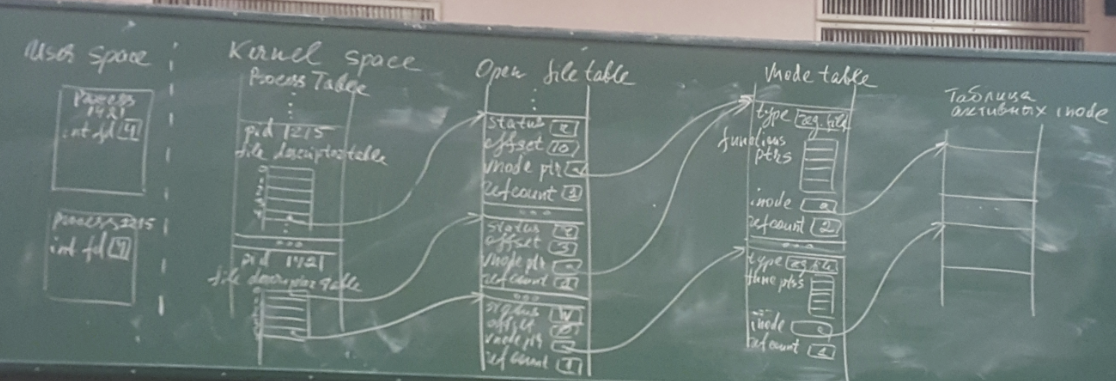
\includegraphics[width=\textwidth]{pic/3.png}
  \caption{Таблицы открытых файлов процессов (фото)}
\end{figure}

Файловый дескриптор – это индекс в таблице, которая  одна на каждый процесс. 
Open File Table – одна на систему.  На каждый открытый файл выделяется структура в этой таблице. 
Несколько процессов могу работать с одним файлом параллельно (не путать "одновременно"). 
inode – это указатель, в котором хранится информация о физическом расположения файла на диске. inode хранятся на диске, но в системе кэшируется информация об inode открытых файлах (таблица активных inode). Эта таблица находится в области данных ядра системы.
Все inode хранятся на диске в массиве фиксированного размера, который называется ilist.
Доступ к файлу осуществляется по номеру inode. Информация о дескрипторах файла (об inode) часто называется мета-данными. Мета данные – это данные о данных.
inode иногда называют номером или индексом (индекс лучше, т.к. это смещение в таблице).

\begin{figure}[H]
  \centering
  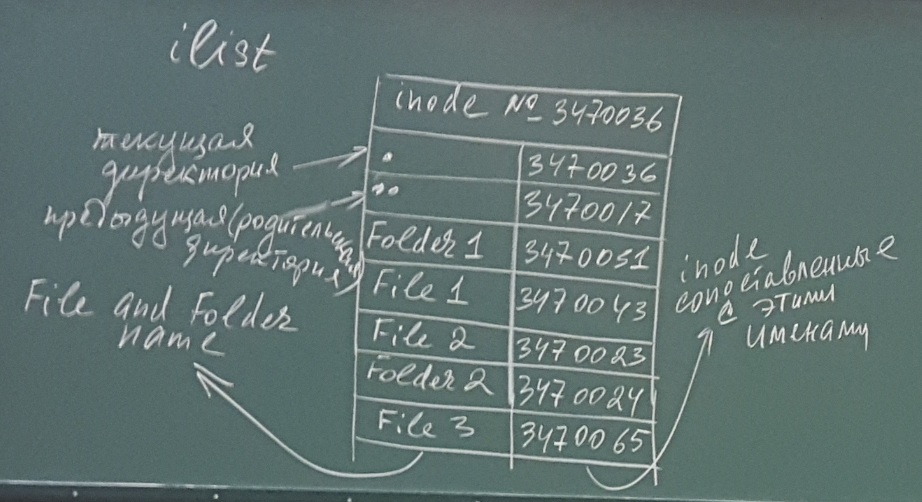
\includegraphics[width=\textwidth]{pic/4.png}
  \caption{pic}
\end{figure}

\begin{figure}[H]
  \centering
  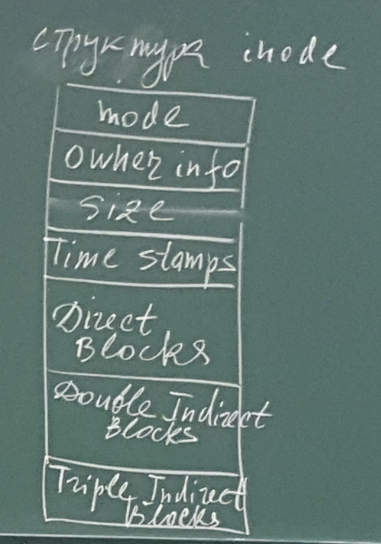
\includegraphics[width=\textwidth]{pic/7.png}
  \caption{Структура inode}
\end{figure}

Файлы хранятся в блоках, а блоки в произвольном порядке в ЖД.

\begin{figure}[H]
  \centering
  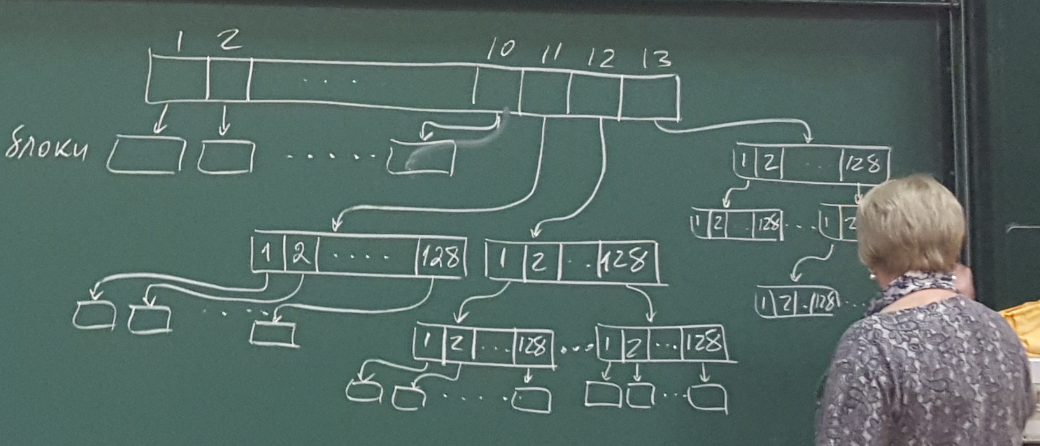
\includegraphics[width=\textwidth]{pic/5.png}
  \caption{pic}
\end{figure}

Через косвенную адресацию позволяет адресовать большие файлы.

По \cite{UNIX_Prof_prog} (стр 151): диски делятся на partition (разделы), а файловая система занимает partition.

\begin{figure}[H]
  \centering
  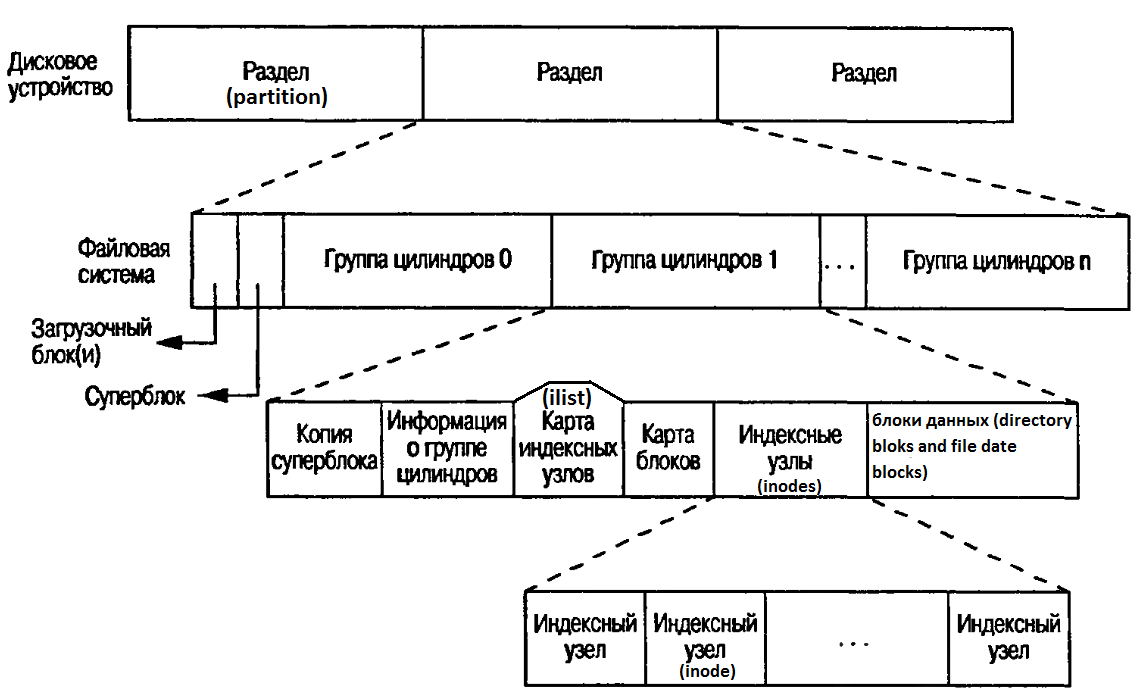
\includegraphics[width=\textwidth]{pic/8.png}
  \caption{Дисковое устройство, разделы и файловая система}
\end{figure}

\begin{figure}[H]
  \centering
  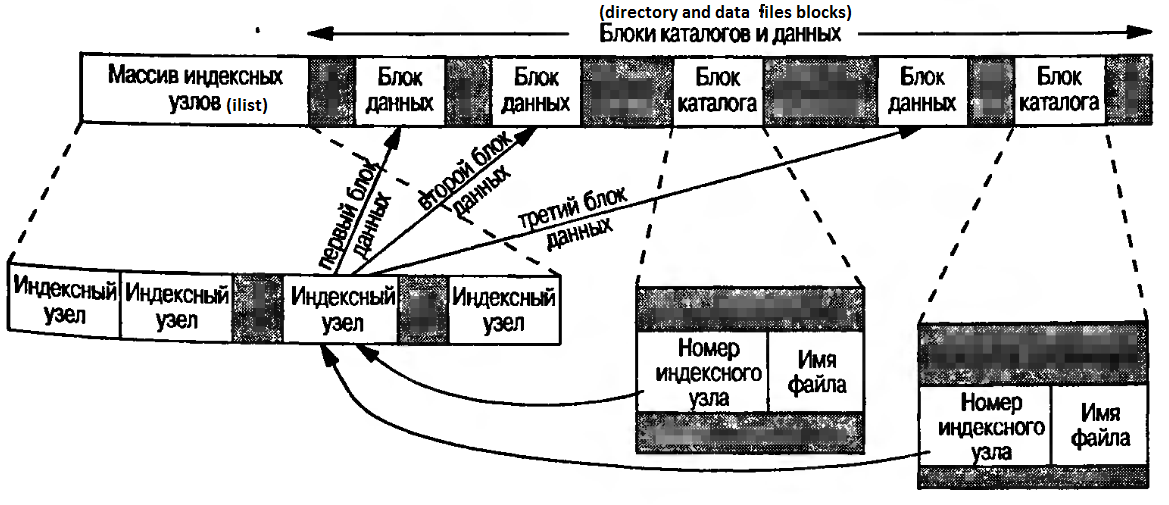
\includegraphics[width=\textwidth]{pic/6.png}
  \caption{Часть группы цилиндров с индексными узлами и блоками данных более детально}
\end{figure}

Директория – таблицы входов.
Зависит от системы.

